\documentclass[14pt]{article}

\usepackage[utf8]{inputenc}
\usepackage[T2A]{fontenc}
\usepackage[english,russian]{babel}

\usepackage{graphicx}
\usepackage{mathtools,amssymb}
\usepackage{amsmath}

\usepackage{hyperref}

\usepackage{subcaption}
% Generate dummy text
\usepackage{lipsum}  
\usepackage{array,multirow}

\def \adl {adl/}

\begin{document}
	Цель: провести исследование возможности восстановления динамики пластового/забойного давления используя инструменты линейной регрессии.
\section{Постановка задачи}
Исследование проведено на примере девятиточечной схемы расстановки скважин (см. рис. \ref{fig:map} ). Исходные данные были получены для 2-х вариантов расчёта:
\begin{enumerate}
	 \item гидродинамическая прокси модель "одна ячейка - одна скважина", одна фаза;
	 \item гидродинамическая модель трещиноватого пласта, две фазы;
\end{enumerate}
Для обоих моделей на скважинах задавался расход жидкости, и рассчитывались значения пластового давления. По периметру расчётной области поддерживалось постоянное пластовое давление равное начальному 10МПа.

\begin{figure}
	\center{\includegraphics[width=14pc]{1.png}}
	\caption{Схема расчётной области}
	\label{fig:map}
\end{figure}

	\section{Двухшаговый метод наименьших квадратов}
Метод оценки параметров эконометрических моделей, в частности систем одновременных уравнений, состоящий из двух этапов (шагов), на каждом из которых применяется метод наименьших квадратов (Википедия).

Шаг 1. Обычным МНК оценивается регрессия факторов X на инструменты X=Z*B + U

Шаг 2. На втором этапе оценивается (также обычным МНК) исходная модель с заменой факторов модели на их оценки, полученные на первом шаге

\begin{equation*} \label{sle}
	\begin{cases}
		p_1^t = \sum_{i=1}^{n} a_{1i}*q_i + \sum_{i\not=1}b_{1i}*p_i + c_1 \\
		p_2^t = \sum_{i=1}^{n} a_{2i}*q_i + \sum_{i\not=2}b_{2i}*p_i + c_2 \\
		...\\
		p_9^t = \sum_{i=1}^{n} a_{9i}*q_i + \sum_{i\not=9}b_{9i}*p_i + c_9 \\
	\end{cases}
\end{equation*}
где n = 9 - кол-во скважин.
Выполняя первый шаг метода находим значения $a_i$ и $c_i$, далее выполняем 2-й шаг и находим $b_i$, при этом подставляя вместо $p_i$ значения найденные на первом шаге. В рамках каждого шага набор уравнений для каждой скважины решается независимо от остальных.
	\section{Результаты вар.1}
В случае первого варианта метрика MAPE для первого и второго шага равны 0.1 и 0.05 соответственно. Динамика исходного и рассчитанного пластового давления представлена на рисунках \ref{fig:1.1_3} - \ref{fig:1.7_9}.
	

\begin{figure}
	\center{\includegraphics[width=30pc]{1-3.png}}
	\caption{Пластовое давление по скважинам 1-3}
	\label{fig:1.1_3}
\end{figure}

\begin{figure}
	\center{\includegraphics[width=30pc]{4-6.png}}
	\caption{Пластовое давление по скважинам 4-6}
	\label{fig:1.4_6}
\end{figure}

\begin{figure}
	\center{\includegraphics[width=30pc]{7-9.png}}
	\caption{Пластовое давление по скважинам 7-9}
	\label{fig:1.7_9}
\end{figure}
метрики по скважинам. Параметры $b_{ji}$ имеют смысл взаимовлияния скважин по давлению, а $a_{ji}$ - взаимовлияния по дебиту. Их этих значений можно составить матрицу коэффициентов, но она не будет симметричной.

	\section{Результаты вар.2}
	Схема расчётно области представлена на рисунке \ref{fig:init_model}, где чёрными точками обозначены места расположения скважин, цветными звёздочками - траектории трещин, цвет звёздочек обозначат принадлежность трещин к одному кластеру.
	При помощи модели были получены значения добычи жидкости и пластового давления, дпо этим данным необходимо настроить регрессионную модель двух/трёхшаговым МНК.
	\begin{figure}
		\center{\includegraphics[width=30pc]{init_model.jpg}}
		\caption{Схема расчётной области}
		\label{fig:init_model}
	\end{figure}
	В случае второго варианта метрика MAPE для первого и второго шага равны 0.1 и 0.05 соответственно. Динамика исходного и рассчитанного пластового давления представлена на рисунках \ref{fig:2.1_3} - \ref{fig:2.7_9}.
	
	\begin{figure}
		\center{\includegraphics[width=30pc]{1-3_2.png}}
		\caption{Пластовое давление по скважинам 1-3}
		\label{fig:2.1_3}
	\end{figure}
	
	\begin{figure}
		\center{\includegraphics[width=30pc]{4-6_2.png}}
		\caption{Пластовое давление по скважинам 4-6}
		\label{fig:2.4_6}
	\end{figure}
	
	\begin{figure}
		\center{\includegraphics[width=30pc]{7-9_2.png}}
		\caption{Пластовое давление по скважинам 7-9}
		\label{fig:2.7_9}
	\end{figure}
	метрики по скважинам
	
\begin{equation} \label{mse}
	J=\frac{w_p}{N_p}\sum_{i=1}^{N_p}{\left(p_c^i-p_f^i\right)^2}+
	\frac{w_{p_w}}{N_{p_w}}\sum_{i=1}^{N_{p_w}}{\left(p_{w\:c}^i-p_{w\:f}^i\right)^2} + f_{pnl},
\end{equation}

	\section{Результаты вар.2, c экзаменом}
	Исследование прогнозных свойств. Временной интервал был разделён на 2 части: обучение - первые 22 месяца, экзамен последние 11 мес. Значения давления представлены ниже.
		
	\begin{figure}
		\center{\includegraphics[width=30pc]{1-3_ex.png}}
		\caption{Пластовое давление по скважинам 1-3}
		\label{fig:2.1_3_ex}
	\end{figure}
	
	\begin{figure}
		\center{\includegraphics[width=30pc]{4-6_ex.png}}
		\caption{Пластовое давление по скважинам 4-6}
		\label{fig:2.4_6_ex}
	\end{figure}
	
	\begin{figure}
		\center{\includegraphics[width=30pc]{7-9_ex.png}}
		\caption{Пластовое давление по скважинам 7-9}
		\label{fig:2.7_9_ex}
	\end{figure}
	Прогнозные свойства для 6 из 9 скв. плохие.
	
	\newpage
	gfgfgfgfg
	\newpage
	
	\section{Регрессия для $\triangle P$. Результаты. Вариант №1 (c экзаменом)}
	В качестве исходной модели была взята однофазная фильтрационная модель слабосжимаемой жидкости. Размер расчётной области 1000м. х 1000м. см. рис. \ref{fig:map9}. Расчётная сетка - прямоугольная, 441 расчётная ячейка. Шаг по времени 1 мес, всего 360 временных шагов.
		\begin{figure}
		\center{\includegraphics[width=16pc]{map1.png}}
		\caption{Схема расчётной области}
		\label{fig:map9}
	\end{figure}
	Моделируемый объект разрабатывается 9-ю скважинами (девятиточечная схема разработки), на скважинах задаются расходы жидкости в виде кусочно постоянных значений. Значения расхода и длительность периодов постоянства генерируются случайным образом. Характерный вид расхода жидкости представлен на рисунке \ref{fig:3.qw_1_9}.
	\begin{figure}[h]
		\center{\includegraphics[width=30pc]{1-9_dP_qw.png}}
		\caption{Пластовое давление по скважинам 1-3}
		\label{fig:3.qw_1_9}
	\end{figure}
	По периметру расчётной области поддерживается постоянное давление 10МПа. При помощи численной модели рассчитываются значения пластового давления вблизи скважин (в ячейках через которые проходят скважины). Характерные карты пластового давления представлены на рисунке \ref{fig:3.press_map}.
	
	\begin{figure}[h]
		\center{\includegraphics[width=30pc]{Press_map.png}}
		\caption{Карты пластового давления для 1, 72 и 240 месяца}
		\label{fig:3.press_map}
	\end{figure}
	
	\textbf{Задача исследования состоит в том что-бы при известных значениях давления и расхода жидкости на скважинах получить упрощённую "прокси" модель и исследовать её прогнозные свойства.}  
	
	С учётом особенности получения исходных данных (при использовании численной математической модели), где на каждом временном шаге решается СЛАУ вида:
	\begin{equation} \label{eq0}
		Ax=b,
	\end{equation}
	где А - разряженная матрица коэффициентов проводимости, x - искомый вектор давлений и b - вектор правых частей содержащий комбинацию известных значений. Матрица А является квадратной матрицей размера n, где n - кол-во расчётных ячеек, векторы x и b также имеют размер n. Так как на практике мы можем измерить значения давления только на скважинах, то из вектора x нам необходимо знать/найти только 9 значений для каждого временного шага. Систему \ref{eq0} при помощи метода частичного исключения можно преобразовать к виду: 
	\begin{equation} \label{eq0.1}
		A_1x_1=b_1,
	\end{equation}
	где $A_1$ - плотная симметричная матрица размерностью 9 на 9, $x_1$ - вектор искомых значений пластового давления и $b_1$ - вектор правой части размером 9. Таким образом исходная система уравнений (состоящая из 441 уравнения) может быть заменена системой из 9 уравнений. Система из 9 уравнений описывает модель ''супер элементов - одна ячейка одна скважина'', которая имеет структуру:
	\begin{itemize}
		 \item связь скважин: "каждая с каждой"
		 \item связь скважин c границей: каждая скважина имеет связь с границей
		 \item каждый элемент имеет аккумуляционную составляющую
	\end{itemize}
	Таким образом для решения обратной задачи (параметрической идентификации при известной структуре) необходимо найти (9*9-9)/2 + 9 + 9 = 54 неизвестных параметра, из которых 36 - имеют смысл проводимости между скважинами/элементами, 9 проводимость между скважинами/блоками и границей, 9 - отвечает за аккумуляционный член.  
	
	\textbf{\textit{Замечание: Для параметрической идентификации исходной модели в общем случае необходимо было подобрать 441 + 441 + 1 = 883 параметра, 441 - значений проницаемости для каждой ячейки, 441 значения эффективной сжимаемости и как минимум ещё один параметр отвечающий за связь аквифера с расчётной областью. Упрощённая модель имеет 54 параметра, что должно положительно сказаться как на адаптации модели так и на стабильности её прогнозных свойств.}}
	     
	Характерный вид уравнения, для j-той скважины/блока в n-тый момент времени:
	\begin{equation} \label{eq1}
		\sum_{i}{ \triangle P_{ij}^n T_{ij}} + \triangle P_{aj}^n T_{aj} + \beta_j (P_j^n - P_j^{n-1}) = q_{j}^n,
	\end{equation}
	где $\triangle P_{ij}^n$ - перепад давления между i и j скважинами/блоками в момент времени $n$, $T_{ij}$ - эффективная проводимость между i и j скважинами/блоками, $\triangle P_{aj}^n = P_a - P_j^n$ и $T_{aj}$ - перепад давление и проводимость между скважиной/блоком и аквифером/границей, $\beta_j$ - эффективная сжимаемость для блока. 
	Если известны значения давления для скважин и расходы жидкости на скважинах, то проводимости можно найти решая СЛАУ вида:
	\begin{equation} \label{m3x1}
		\begin{vmatrix}
			D^1& C^1\\
			D^2& C^2 \\
			\vdots&\vdots\\
			D^n& C^n
		\end{vmatrix}
		* 
		\begin{vmatrix}
			T\\
			\beta
		\end{vmatrix}
		=
		\begin{vmatrix}
			q^1\\
			q^2\\
			\vdots\\
			q^n
		\end{vmatrix},
	\end{equation}
	где $D^n$ - матрица депрессий между скважинами, $C^n$ - диагональная матрица разности давлений на текущем ($n$) и предыдущем ($n-1$) временных шагах, $T$ - вектор эффективной проводимости, $\beta$ - вектор эффективной сжимаемости ("псевдосжимаемости"), $q^n$ - вектор расходов жидкости.
	
	
	В общем случае СЛАУ будет/должна быть переопределенной, решение получается при помощи МНК. Ранг матрицы разности давлений должен быть равен 54, иначе существует бесконечное число решений. Если при составление матрицы разности давлений её ранг меньше кол-ва неизвестных, то  можно/нужно огрублять модель (менять её структуру), таким образом чтобы возможно было получить решение (\textbf{дальнейшие исследования}). 
	
Период разработки был разбит на 2 интервала: период адаптации 72 мес. и период экзамена 288 мес. равные 20\% и 80\% от общего периода моделирования. Используя \ref{m3x1}, были найдены параметры $T$ и $\beta$. При использовании найденных параметров были рассчитаны значения пластового давления на прогноз (период экзамена). Динамика пластового давления представлена на рисунках \ref{fig:3.1_3} - \ref{fig:3.7_9}.
	
	\begin{figure}[h]
		\center{\includegraphics[width=30pc]{1-3_dP.png}}
		\caption{Пластовое давление по скважинам 1-3}
		\label{fig:3.1_3}
	\end{figure}

	\begin{figure}[h]
		\center{\includegraphics[width=30pc]{4-6_dP.png}}
		\caption{Пластовое давление по скважинам 4-6}
		\label{fig:3.4_6}
	\end{figure}

	\begin{figure}[h]
		\center{\includegraphics[width=30pc]{7-9_dP.png}}
		\caption{Пластовое давление по скважинам 7-9}
		\label{fig:3.7_9}
	\end{figure}
	
	 Метрики MAPE для периодов адаптации и экзамена составляют 0,9\% и 23,5\% соответственно. Следовательно можно сделать вывод о том, что модель хорошо адаптированна, но имеет не удовлетворительные прогнозные свойства. Рассмотрим значения метрик по скважинам (см. таб. \ref{tabl:well_mape}) 
	\begin{table}[h!]
		\caption{Метрики для периода адаптации и прогноза}	
		\label{tabl:well_mape}	
		\begin{center}
		\begin{tabular}{c|c|c|c|c}
		\hline
		Cкв. № & MAPE адп., \% & MAPE экз, \% & MSE адп., MПа & MSE экз, MПа \\
		\hline
 		1 & 0.4 & 15.7 & 0.1 & 1.3 \\
		2 & 0.9 & 1.7 & 0.1 & 0.2 \\
		3 & 0.5 & 0.7 & 0.1 & 0.1 \\
		4 & 0.5 & 184.9 & 0.1 & 5.3 \\
		5 & 1.9 & 2.2 & 0.2 & 0.3 \\
		6 & 0.9 & 1.8 & 0.1 & 0.2 \\
		7 & 0.7 & 1.7 & 0.1 & 0.1 \\
		8 & 1.1 & 1.8 & 0.1 & 0.2 \\
		9 & 0.9 & 1.0 & 0.1 & 0.1 \\
		\hline
	
		\end{tabular}
		\end{center}
	\end{table}
	
	Из таблицы видно, что основной вклад метрику для периода экзамена вносит скважина № 4, рассмотрим её подробнее. На периоде адаптации динамика пластового давления и расход жидкости были практически постоянными, что не позволило достаточность её настроить.
	
	\begin{table}[h!]
	\caption{Коэффициенты вариации для фазовых переменных}	
	\label{tabl:well_var}	
	\begin{center}
		\begin{tabular}{c|c|c|c|c}
		\hline
		Cкв. № & VAR адп. P \% & VAR экз. P \% & VAR адп. Q & VAR экз. Q \\
		\hline
		1 & 0.02 & 3.66 & 0.0 & 0.08 \\ 
		2 & 1.63 & 2.45 & 0.02 & 0.03 \\ 
		3 & 5.53 & 4.76 & 0.08 & 0.05 \\ 
		4 & 0.04 & 9.39 & 0.0 & 0.14 \\ 
		5 & 1.06 & 7.23 & 0.02 & 0.06 \\ 
		6 & 2.67 & 3.11 & 0.04 & 0.02 \\ 
		7 & 5.19 & 0.88 & 0.08 & 0.0 \\ 
		8 & 1.15 & 5.54 & 0.02 & 0.06 \\ 
		9 & 11.76 & 1.98 & 0.19 & 0.02 \\ 
		\hline
		\end{tabular}
	\end{center}
	\end{table}

Плохие прогнозные свойства для 4-й скважины можно объяснить малым коэффициентом вариации расхода жидкости, а следовательно, и пластовым давлением на периоде адаптации. На экзаменационном периоде наоборот коэффициент вариации расхода жидкости максимальный, что приводит к большим отклонениям расчётных значений от эталонных.
	Значения $T$ представлены в \ref{m3x2} в виде верхней треугольной матрицы
\begin{equation*} \label{m3x2}
\begin{vmatrix}
 * &  0.0107 &  0.0019 & -0.0148  & 0.0024 & -0.0002 &   0.0018 &  -0.0016  & 0.0004 \\
  & *  & 0.0134  & 0.0061 &  0.013   & 0.0055  & 0.0014  & 0.0038 &  0.0012 \\
 &   & * & -0.0003  & 0.0062 &  0.0107  & -0.0001  & 0.0004  & 0.0013 \\
  &  &   & * &  0.0077  & 0.0006 &  0.006  &  0.0023 &  . \\
  &     &  &  & * &  0.0136  & 0.0049  & 0.0127  & 0.0055 \\
  &   &   &   &  & *  & . &  0.0049  & 0.0106 \\
   &  &   &   &   &  &  *  & 0.0111  & 0.0008 \\
  &   &  &  &   &  &  & * &  0.0139 \\
   &  &    &  &   &  &  &  & *
\end{vmatrix}
\end{equation*}
Как видно некоторые значения меньше 0, что с точки зрения физики невозможно, необходимо доработать алгоритм в плане регуляризации. Кроме того с учётом того, что исходная модель имела одно значение проницаемости для всех ячеек, логичным  было бы равенство значений проводимости для симметричных скважин (1, 3, 7, 9 - угловые), из таблицы видно что они отличаются, хотя значения в большей части близки друг к другу. 

Другой вариант адаптации:
\begin{equation*} \label{m3x3}
	\begin{vmatrix}
* &1.85 &0.98 &1.68 &1.31 &0.04 &1.83 &0.15 &0.24\\
&* &1.45 &0.87 &2.17 &0.51 &0.09 &0.14 &-0.23\\
& &* &0.86 &1.59 &2.48 &-0.04 &0.08 &0.54\\
& & &* &2.81 &0.63 &0.2 &1.09 &0.09\\
& & & &* &2.51 &0.93 &2.53 &1.09\\
& & & & &* &-0.45 &1.0 &1.77\\
& & & & & &* &1.49 &-0.18\\
& & & & & & &* &1.74\\
& & & & & & & &*\\
\end{vmatrix}
\end{equation*}

Погрешность/ошибка восстановленных параметров \%.
\begin{equation*} \label{m3x4}
	\begin{vmatrix}
		* &17.2 &74.4 &60.4 &23.9 &1632.8 &47.0 &339.3 &170.2\\
		&* &26.4 &39.2 &11.5 &63.8 &451.9 &217.8 &102.3\\
		& &* &91.0 &22.2 &27.3 &2011.4 &742.4 &93.1\\
		& & &* &12.1 &113.5 &477.3 &51.2 &472.6\\
		& & & &* &13.4 &41.6 &13.1 &22.0\\
		& & & & &* &189.8 &52.2 &24.9\\
		& & & & & &* &42.8 &281.2\\
		& & & & & & &* &20.9\\
		& & & & & & & &*
	\end{vmatrix}
\end{equation*}

\begin{figure}[h]
	\center{\includegraphics[width=25pc]{пров_пог.png}}
	\caption{Кросс-плот зависимость погрешности параметра от его значения}
	\label{fig:err_vs_val}
\end{figure}

Исходные значения:
\begin{equation*} \label{m3x3_init}
	\begin{vmatrix}
		* &5.7 &0.23 &5.7 &1.77 &0.15 &0.23 &0.15 &0.03\\
		&* &5.7 &1.77 &6.13 &1.77 &0.15 &0.29 &0.15\\
		& &* &0.15 &1.77 &5.7 &0.03 &0.15 &0.23\\
		& & &* &6.13 &0.29 &5.7 &1.77 &0.15\\
		& & & &* &6.13 &1.77 &6.13 &1.77\\
		& & & & &* &0.15 &1.77 &5.7\\
		& & & & & &* &5.7 &0.23\\
		& & & & & & &* &5.7\\
		& & & & & & & &*\\
	\end{vmatrix}\quad
	\begin{vmatrix}
		48,4  \\
		30,3  \\
		48,4  \\
		30,3  \\
		7,1  \\
		30,3  \\
		48,4  \\
		30,3  \\
		48,4  \\
	\end{vmatrix}\quad
	\begin{vmatrix}
	94,8 \\
	104,4 \\
	94,8 \\
	104,4 \\
	116,7 \\
	104,4 \\
	94,8 \\
	104,4 \\
	94,8 \\
	\end{vmatrix}
\end{equation*}

.\\
.\\
.\\
.\\
.\\
.................\\
Как видно из рисунка \ref{fig:err_vs_val} наиболее высокие значения проводимости определяются наиболее точно.

\textit{Далее планирую исследовать и рассчитывать погрешности для восстановленных параметров, с учётом коэффициентов вариации и ковариации для исходных данных}

	\newpage
	
	\section{Регрессия для $Q_w$. Результаты. Вариант №1 (c экзаменом), снижение размерности}

Исходные (фактические) данные получены из однофазного симулятора, модель см. выше. Прокси модель берётся в виде линейной регрессии. Решается уравнение вида:
 \begin{equation}\label{qw_reg}
 		p_i^n = \sum_{i=1}^{N}a_i q_{w i}^n + b_i,
 	\end{equation}
 	где $a_i$ и $b_i$ искомые параметры модели, $q_w$ - добыча жидкости, $p$ - пластовое давление, $i$ - номер скважины, $n$ - номер временного шага.
 	
 	Для оценки прогнозных свойств прокси модели временной интервал разбивается на два периода - период адаптации и период экзамена. Периоды занимают 30\% и 70\% от общего периода моделирования. \textbf{Целью данной задачи является исследование применимости методов сокращения размерности на примере "метода главных компонент" (PCA).} 
 	
 	Дано: расходы жидкости на скважинах и пластовые давления вблизи скважин (в расчётных ячейках). Расходы жидкости выбирались таким образом что-бы получение решения для полноценной регрессионной модели было невозможным или заведомо имело плохие прогнозные свойства (постоянные значения расходов на некоторых скважинах). Под полноценной моделью понимается уравнение \ref{qw_reg} содержащее 9 слагаемых - 9 неизвестных параметров $a$. Для получения решения использовался приём снижения размерности исходных данных. Для полученного решения исследовались прогнозные свойства. Динамика расходов жидкости на скважинах представлен на рисунке \ref{fig:exmpl7qw}.
 	
 	\begin{figure}
 		\centering
 		\includegraphics[width=1.0\linewidth]{exmpl_7_qw}
 		\caption{Динамика расхода жидкости на скважинах]}
 		\label{fig:exmpl7qw}
 	\end{figure}
 	
 	Расходы жидкости на скважинах были заданы кусочно-постоянными функциями. В период адаптации на 6-ти случайных скважинах значения расходов существенно меняли значение. Для оставшихся 3х скважин первые 100 месяцев были заданы постоянные расходы жидкости. Период адаптации составлял 108 месяцев, что больше периода постоянной работы 3-х скважин. Это было сделано намеренно, так как при периоде постоянства расходов большем или равном периоду адаптации полноценная регрессионная модель не работает. 
 	
 	%линейной регрессии (LR) и модели авторегрессии и распределённого лага (ADL)
 	
 	На рисунках \ref{fig:ppllinregw1} и \ref{fig:ppladlw1} представлена динамика пластового давления для первой скважины. На рисунках также приведены адаптированные и прогнозные значения давления, доверительные интервалы значений и динамика относительной погрешности расчётного значения давления. Рисунки \ref{fig:ppllinregw1} и \ref{fig:ppladlw1} приведены для двух аппроксимирующих LR и ADL моделей соответственно.
 	
 \begin{figure}
 	\centering
 	\includegraphics[width=0.9\linewidth]{ppl_lin_reg_w1}
 	\caption{Динамика пластового давления, LR}
 	\label{fig:ppllinregw1}
 \end{figure}
 
 	На рисунке \ref{fig:ppllinregw1} изображена расчётная динамика давления для двух вариантов исходных данных с разной размерностью равной 7 и 8 на графике изображены зелёной и синей линиями соответственно. 
 
 \begin{figure}
 	\centering
 	\includegraphics[width=0.9\linewidth]{ppl_adl_w1}
 	\caption{Динамика пластового давления, ADL}
 	\label{fig:ppladlw1}
 \end{figure}
 
 	На рисунке \ref{fig:ppladlw1} аналогично представлена расчётная динамика давления получена при помощи ADL модели для двух вариантов исходных данных, но с размерностью равной 16 и 18 (на графике изображены зелёной и синей линиями соответственно).
 	
 	Из графиков видно, что относительная погрешность расчётных значений давления выше для вариантов с большей размерностью. Кроме того для модели ADL происходит постепенный рост погрешности с течением времени, что объясняется накоплением ошибки. Тем не менее расчётное значение для варианта с большей размерностью (метрика MAPE) ближе к фактическому для модели ADL, но погрешность её выше.  
 
 	На рисунках \ref{fig:ppllinregw1} и \ref{fig:ppladlw1} в качестве примера были приведены результаты для одного расчёта для одной скважины. С целью набора статистики для оценки прогнозных свойств модели было выполнено моделирование 128 сценариев, каждый сценарий прогноза исследовался для 9 возможных вариантов снижения размерности исходных данных. Для модели LR размерность данных соответствует количеству параметров которые необходимо подобрать. 
 	На рисунке \ref{fig:mapevsndimlr} представлена зависимость усредненной метрики MAPE от размерности преобразованных исходных данных для модели линейной регрессии (LR). 

\begin{figure}
	\centering
	\includegraphics[width=0.9\linewidth]{mape_vs_ndim_lr}
	\caption{Зависимость точности адаптации и прогноза от размерности исходных данных, модель LR}
	\label{fig:mapevsndimlr}
\end{figure}

	На рисунке \ref{fig:mapevsndimadl} представлена зависимость усредненной метрики MAPE от размерности преобразованных исходных данных для модели линейной регрессии (ADL).

\begin{figure}
	\centering
	\includegraphics[width=0.9\linewidth]{mape_vs_ndim_adl}
	\caption{Зависимость точности адаптации и прогноза от размерности исходных данных, модель ADL}
	\label{fig:mapevsndimadl}
\end{figure}

Из рисунка видно, что ошибка адаптации и прогноза синхронно снижается с увеличением размерности исходных данных вплоть до значения равного 7. Далее снижение среднего значения MAPE для периода адаптации практически прекращается. Для прогноза, наоборот, начинается заметный рост метрики (снижение точности прогноза). Кроме того, при количестве параметров больше 8 появляются сценарии прогноза для которых ошибка составляет более 100\%, для таких сценариев возрастает с увеличением кол-ва параметров (жёлтые столбцы на рис. \ref{fig:mapevsndim5}). На графике также приведены значения средней относительной погрешности расчётных значений давления для периодов адаптации и прогноза. Относительная ошибка для периода адаптации является относительно не большой (менее 2\%). Для прогнозного периода средняя относительная ошибка растёт с увеличением кол-ва переменных, наиболее резкий рост наблюдается при превышении критического значения кол-ва переменных равного 7.  Подобное поведение ошибки адаптации и прогноза свидетельствует о том, что сложность модели должна выбираться согласно "разрешающей способности" исходных данных. В нашем примере для описания поведения динамики давления хватит модели с 7 параметрами, при этом прогнозные свойства являются удовлетворительными. При превышении кол-ва переменных ухудшаются не только прогнозные свойства модели но и растёт погрешность получаемых решений. 

На рисунке \ref{fig:mapevsndim1} представленный осреднение значения, интересным также является распределение ошибки для разных сценариев. На рисунках \ref{fig:histadp1} - \ref{fig:histprog5} представлены гистограммы распределения метрики MAPE для 128 сценариев. 

Из профилей гистограмм видно что при росте количества переменных снижается как сами значения ошибок, так и их дисперсия. 

	\newpage

\section{Двухфазная ADL модель. Результаты. Вариант №1 (обучение + экзамен, модель из статьи с нейросетями)}
Задача: на примере синтетической модели из статьи в Вестнике ТЮмГУ (про нейросети, 2023) оценить возможность применения модели ADL для адаптации и прогнозирования забойного давления и дебита нефти. На рисунке \ref{fig:map_init_perm} представлена схема моделируемого объекта (расположение скважин и карта проницаемости). 
\begin{figure}
	\centering
	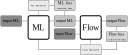
\includegraphics[width=0.9\linewidth]{fig1.png}
	\caption{Карта проницаемости исходной модели}
	\label{fig:map_init_perm}
\end{figure}

Модель двухфазная, значение вязкостей 1 и 10 для воды и нефти соответственно. В начальный момент времени пласт полностью заполнен нефтью. 

\subsection{ADL модель, 1 фаза}
При моделировании фильтрационных процессов используют численные фильтрационные модели, в которых на каждом временном шаге решается СЛАУ вида: 

\begin{equation} \label{eq01}
	Ap^n=bp_a + \beta^*p^{n-1} + q^n,
\end{equation}

Для использования метода частичного (блочного) исключения представим систему \ref{eq01} в виде:

\begin{equation} \label{eq02}
	\begin{bmatrix}
		A_{11} & A_{12} \\
		A_{21} & A_{22}
	\end{bmatrix}
	\begin{bmatrix}
		 \mathbf { p_1^n } \\
		 \mathbf { p_2^n }
	\end{bmatrix}
	=
	\begin{bmatrix}
		 \mathbf {b_1} \cdot p_a \\
		 \mathbf {b_2} \cdot p_a 
	\end{bmatrix}
	+
	\begin{bmatrix}
		 \boldsymbol{\beta_1^*}\circ  \mathbf {p_1^{n-1}} \\
		  \boldsymbol{\beta_2^*}\circ  \mathbf {p_2^{n-1}} 
	\end{bmatrix}
	+
	\begin{bmatrix}
		0 \\
		\mathbf{q^n}
	\end{bmatrix},
\end{equation}
где $A_{11}$ - матрица коэффициентов размерностью $m_1*m_1$, $A_{22}$ - матрица коэффициентов  размерностью $m_2*m_2$, $A_{12}$ и $A_{21}$ - матрица коэффициентов размерностью $m_1*m_2$ и $m_2*m_1$, причём $A_{12}=A_{21}^T$, $\mathbf{p_1^n}$ - вектор пластового давления в ячейках не содержащих скважины, $\mathbf{p_2^n}$ - пластовое давление в ячейках через которые проходят скважины, $n$ - номер временного шага, $\mathbf{b}$ - вектор характеризующий связь расчётных ячеек в границей, $p_a$ - давление на границе (в аквифере), $\mathbf{q^n}$ - вектор расходов жидкости на скважинах. 

При учёте того, что в реальных условия нам известны значения параметров (фазовых переменных, давления) только в местах расположения скважин, другими словами нам достоверно известны только значения $p_w$. Преобразуем систему \ref{eq02} таким образом, чтобы в качестве неизвестных остались только непосредственно измеряемые величины. Получим:
 
\begin{equation} \label{eq03}
\mathbf { p_1^n } = A_{11}^{-1}\left(\mathbf{b_1} \cdot p_a +
\boldsymbol{\beta_1^*} \circ  \mathbf {p_1^{n-1}} - A_{12} \mathbf {p_2^n}  \right)
\end{equation}

\begin{equation*} \label{eq04}
	A_{21} \mathbf { p_1^n } + A_{22} \mathbf {p_2^n} =\mathbf{b_2} \cdot p_a +
	\boldsymbol{\beta_2^*} \circ  \mathbf {p_2^{n-1}} + \mathbf{q^n}.
\end{equation*}
Подставим в него уравнение \ref{eq03}, получим:
\begin{equation*} \label{eq05}
	(A_{22} - A_{21} A_{11}^{-1} A_{12})\mathbf {p_2^n} = \mathbf{b_2} \cdot p_a +
	\boldsymbol{\beta_2^*} \circ  \mathbf {p_2^{n-1}} + \mathbf{q^n} - A_{21} A_{11}^{-1}\left(\mathbf{b_1} \cdot p_a +
	\boldsymbol{\beta_1^*} \circ  \mathbf {p_1^{n-1}} \right).
\end{equation*}
Обозначим $A_{i2} = (A_{22} - A_{21} A_{11}^{-1} A_{12})^{-1}$ - квадратная плотная матрицы размером $m_2*m_2$ (индекс $i$ - означает "обратная" (inverse)).

\begin{equation} \label{eq06}
	\mathbf {p_2^n} = A_{i2} (\mathbf{b_2} -A_{21} A_{11}^{-1} \mathbf{b_1})\cdot p_a +
	A_{i2} \left(\boldsymbol{\beta_2^*} \circ  \mathbf {p_2^{n-1}}\right) + A_{i2} \mathbf{q^n}
	- 	A_{i2} \left(A_{21} A_{11}^{-1} \left(\boldsymbol{\beta_1^*} \circ  \mathbf {p_1^{n-1}}\right)\right).
\end{equation}

Учитывая тот факт, что фактические замеры давления выполняются только в скважинах, по сути являются замерами забойного давления, выразим пластовое давление через забойное. Их уравнения 
\begin{equation*} \label{eq07}
q_j^n = w_j\left(p_j^n - {p^n_w}_j \right)
\end{equation*}
выразим $p_j^n$, получим:
\begin{equation*} \label{eq08}
p_j^n = {p^n_w}_j + \frac{q_j^n}{w_j},
\end{equation*}
подставим в \ref{eq06}, получим:

\begin{eqnarray} \label{eq09}
	\mathbf {p_w^n} = A_{i2} (\mathbf{b_2} -A_{21} A_{11}^{-1} \mathbf{b_1})\cdot p_a + \nonumber \\ 
	+ A_{i2} \left(\boldsymbol{\beta_2^*} \circ  \mathbf {p_w^{n-1}}\right)
	+ A_{i2} \left(\boldsymbol{\beta_2^*} \circ   \frac{1}{\mathbf{w}} \mathbf{q^{n-1}} \right)+  \nonumber \\ 
	+ \left(A_{i2} -  \frac{1}{\mathbf{w}}\right) \mathbf{q^n}
	- 	A_{i2} \left(A_{21} A_{11}^{-1} \left(\boldsymbol{\beta_1^*} \circ  \mathbf {p_1^{n-1}}\right)\right).
\end{eqnarray}

или 

\begin{eqnarray} \label{eq010}
	\mathbf {p_w^n} = A  \mathbf {p_w^{n-1}}
	+ B \mathbf{q^n} + C \mathbf{q^{n-1}} + D p_a  
	- 	A_{i2} \left(A_{21} A_{11}^{-1} \left(\boldsymbol{\beta_1^*} \circ  \mathbf {p_1^{n-1}}\right)\right).
\end{eqnarray}

последнее слагаемое при использовании \ref{eq03} можно представить как сумму произведений коэффициентов на значения забойного давления, дебита жидкости, начального и граничного условия. 

\begin{eqnarray} \label{eq010}
	\mathbf {p_w^n} = A  \mathbf {p_w^{n-1}}
	+ B \mathbf{q^n} + C \mathbf{q^{n-1}} + D' p_a  
	+ \sum_{i=1}^{n-2}{\left(F_i*q_w^i + G_i*p_w^i\right)}.
\end{eqnarray}

То есть значение забойного давления на некотором шаге равняется линейной комбинация предыдущих значений забойного давления и расходов жидкости. Сократим количество временных шагов взяв размер окна равный двум шагам (текущий и предыдущий). Выбор ширины окна большего размера приведёт к повышению точности адаптации (большее кол-во настраиваемых параметров), но и к снижению обусловленности задачи. Таким образом остановимся на СЛАУ вида: 
\begin{eqnarray} \label{eq0_sustem_adl}
	\mathbf {p_w^n} = A  \mathbf {p_w^{n-1}}
	+ B \mathbf{q^n} + C \mathbf{q^{n-1}} + D p_a.
\end{eqnarray}
каждое уравнение имеет вид:
\begin{eqnarray} \label{eq0_adl_adl}
{p_w^n}_j = \sum_{i=1}^{m2}{\left( a_i {p_w^{n-1}}_i
+ b_i q_i^n + c_i q^{n-1}_i\right)} + d_i p_a.
\end{eqnarray}
Преобразуем к виду характерному для ADL модели:
\begin{eqnarray} \label{eq0_adl_adl}
	\triangle p_w^n={p_w^n}_j -  {p_w}_j^{n-1}= \left(a_j-1\right){p_w}_j^{n-1} + \sum_{i=1, i\neq j}^{m_2}{a_i {p_w^{n-1}}_i}
		+ \sum_{i=1}^{m_2}{\left( b_i q_i^n + c_i q^{n-1}_i\right)} + d_i p_a.
\end{eqnarray}
Полученное уравнение представляет собой структурную форму ADL модели полученную из полной СЛАУ фильтрационной модели (с учётом ряда допущений). Полученная структурная форма справедлива для каждой строки в \ref{eq0_sustem_adl}. Решение полученного уравнения находится при помощи МНК. Найденные коэффициенты позволяют выполнять прогнозные расчёты. 

Полученная модель была протестированная примере 3-х моделей разной степени сложности.
\begin{enumerate}
	\item гидродинамическая прокси модель "одна ячейка - одна скважина", одна фаза;
	\item Модель зонально неоднородного пласта ;
	\item гидродинамическая модель трещиноватого пласта, две фазы;
\end{enumerate}

\begin{figure}
	\begin{subfigure}{\textwidth}
		\centering
		\includegraphics[width=0.8\textwidth]{\adl pic3.png}
		\caption{}
		\label{fig:p_a}
	\end{subfigure}
	\begin{subfigure}{\textwidth}
		\centering
		\includegraphics[width=0.8\textwidth]{\adl pic4.png}
		\caption{}
		\label{fig:p_b}
	\end{subfigure}
	\begin{subfigure}{\textwidth}
		\centering
		\includegraphics[width=0.8\textwidth]{\adl pic5.png}
		\caption{}
		\label{fig:p_c}
	\end{subfigure}
	\caption{Динамика давления на забое скважин: фактические, адаптированные и прогнозные значения}
	\label{fig:m1_press_abc}
\end{figure}

\begin{table}[h!]
	\caption{Метрика MAPE и RMSE по скважинам}	
	\label{tabl:MAPE_RMSE}	
	\begin{center}
		\begin{tabular}{|c||c|c||c|c|}
			\hline
			\multirow{2}{*}{№} & \multicolumn{2}{c||}{MAPE, \%} & \multicolumn{2}{c|}{RMSE, МПа} \\\cline{2-5}
			& адп. & экз. & адп. & экз. \\
			\hline
			1 & 0,6 & 6,1 & 0,03 & 0,22 \\
			\hline
			2 & 0,5 & 1,8 & 0,08 & 0,35 \\
			\hline
			3 & 0,4 & 3,7 & 0,01 & 0,27 \\
			\hline
			4 & 0,3 & 1,4 & 0,08 & 0,27 \\
			\hline
			5 & 0,4 & 11,7 & 0,02 & 0,36 \\
			\hline
			6 & 0,5 & 2,3 & 0,09 & 0,46 \\
			\hline
			7 & 0,2 & 3,0 & 0,01 & 0,12 \\
			\hline
			8 & 0,3 & 0,5 & 0,09 & 0,16 \\
			\hline
			9 & 0,3 & 2,5 & 0,02 & 0,15 \\
			\hline
		\end{tabular}
	\end{center}
\end{table}







	\newpage
	
\begin{eqnarray} \label{mse_1}
	J=\frac{w_p}{N_p}\sum_{i=1}^{N_p}{\left(p_c^i-p_f^i\right)^2}+ \\
	 + \frac{w_{p_w}}{N_{p_w}}\sum_{i=1}^{N_{p_w}}{\left(p_{w\:c}^i-p_{w\:f}^i\right)^2} + \\
	+ \frac{w_{q_w}}{N_{q_w}}\sum_{i=1}^{N_{q_w}}{\left(q_{w\:c}^i-q_{w\:f}^i\right)^2} + \\
	 + \frac{w_{\sigma_w}}{N_{\sigma_w}}\sum_{i=1}^{N_{\sigma_w}}{\left(\sigma_{w\:c}^i-\sigma_{w\:f}^i\right)^2} +  f_{pnl},
\end{eqnarray}


\begin{equation}\label{grad}
	\begin{matrix}
	\frac{\partial J}{\partial u_k} = 2w_p \frac{1}{N_p}\sum_{i=1}^{N_p}({p_c^i-p_f^i}) \frac{\partial p_c^i}{\partial	u_k}+ \\	
	+ 2w_{p_w}\frac{1}{N_{p_w}}\sum_{i=1}^{N_{p_w}}({p_{w\:c}^i-p_{w\:f}^i}) \frac{\partial p_{w\:c}^i}{\partial u_k}+ \\
	+ ... + 	\\
		+ 2w_{q_w}\frac{1}{N_{q_w}}\sum_{i=1}^{N_{q_w}}{\left(q_{w\:c}^i-q_{w\:f}^i\right)}\frac{\partial
			q_{w\:c}^i}{\partial u_k} \rightarrow 0
			\end{matrix}
\end{equation}

\begin{equation}
	J = \sum_{k=1}^K \frac{w_k}{N_k}\sum_{i=1}^{N_k}(x_i^f - x_i^c)^2	
\end{equation}

\begin{equation}
	q_{j \:m} = \kappa_j\sigma_j(p_j^2-p_{w\:j}^2)
\end{equation}

\begin{equation}
	\nabla \sigma \nabla p^2= m h \frac{\partial p}{\partial t} + \delta(x,y)
\end{equation}

\begin{equation} \label{bc}
	\delta(x,y)  = \left\{\begin{array}{crl}
		0, \;\mbox{при}\;(x,y) \notin\ \Gamma_{in}\cup\Gamma_{out},\\
		q_{j\:m}, \;\mbox{при}\;(x,y) \in \Gamma_{in},\\
		q_{aq \: m}, \;\mbox{при}\;(x,y) \in \Gamma_{out},
	\end{array}\right.
\end{equation}

\begin{equation}
	p = p_0, \quad \mbox{при} {\:} t=0
\end{equation}

\begin{equation*}
	q_{aq \:m} = \lambda \sigma|_{_{\Gamma_{out}}} (p_{a}^2 - p^2|_{_{\Gamma_{out}}}), \\
\end{equation*}

\begin{equation*}
	p_{aq} = p_0, \quad \mbox{при} {\:} t=0
\end{equation*}
вждалывджал

	$p$ - пластовое давление;
	
	$p_w$ - забойное давление;
	
	$q_m$ - массовый расход;
	
	$\sigma = \sigma(x,y)$ - гидропроводность;
	
	$\kappa_j$ - коэффициент связи с пластом для j-той скважины;
	
	$\lambda$ - продуктивность контура питания (аквифера).
	
	$m$ - пористость.
	
	$h$ - эффективная толщина.
	
	
	\begin{thebibliography}{20}
		
		\bibitem{raf} R. Holanda, "A State-of-the-Art Literature Review on Capacitance
		Resistance Models for Reservoir Characterization
		and Performance Forecasting" Rafael Wanderley de Holanda, Eduardo Gildin, Jerry L. Jensen, Larry W. Lake and C. Shah Kabir. Energies 2018, 11(12), 3368; https://doi.org/10.3390/en11123368
		
		\bibitem{kos} V. P. Kosyakov, "Structural and Parametric Identification
		of an Aquifer Model for an Oil Reservoir". Lobachevskii J. Math.
		{\bf 41}, 1242--1247 (2020).
		
		\bibitem{bas} K. S. Basniev, N. M. Dmitriev, R. D. Kanevskaya, and V. M. Maksimov,
		\textit{Underground hydromechanics}. M.-Izhevsk: Institute for
		Computer Research, 2006 [in Russian].
		
		\bibitem{azi} H. Aziz and E. Settari, \textit{Mathematical modeling of reservoir systems}.
		M.-Izhevsk: Institute for Computer Research, 2004 [in Russian].
		
		\bibitem{opt} V. P. Kosyakov and S. P. Rodionov, "Optimal control of wells on the basis
		of two-phase filtration equations", Proceedings of MIPT {\bf 8} (3),
		79--90 (2016).
		
		\bibitem{leg} V. P. Kosyakov and  D. Yu. Legostaev, "Using elements of machine learning to
		solve the inverse problem of reconstructing the hydraulic 
		conductivity feld for a fltration problem", Tyumen State University
		Herald. Physical and Mathematical Modeling. Oil, Gas, Energy {\bf 8}
		(2 (30)), 129--149.
		
	\end{thebibliography}
	
\end{document}
